

\section{Artifacts and Outliers in Large-Scale Training}
\label{app:sec:artifacts}

This section provides a discussion about the emergence of artifacts and outliers that has recently been observed in the training of large models in both the LLM~\citep{an2025systematic} and the visual domains~\citep{darcet2024vision}. 
Borrowing the definition from \citet{an2025systematic}, outliers are typically characterized as network's activations whose values deviate significantly from the average of their distribution. %
During the training of DINOv3, we identified such outliers at different levels: some occurring at the patch level and others at the feature dimension level. 
We discuss bellow the different types of outlier observed, their impact on the training and results. 
We also discuss our different attempts at fixing them and our first conclusions. 

\subsection{High-Norm Patch Outliers}
 
\citet{darcet2024vision} discovered that patch outliers negatively affect performance in DINOv2. 
These outliers are primarily characterized as high-norm tokens, often located in low-information background regions of an image. 
These tokens are observed to play a key role in the internal communication between patches and the CLS token. 
Additionally, this phenomenon affects other models as well, whether trained with supervision or not, such as CLIP~\citep{radford2021learning}.
When scaling to a 7B model, we observe the emergence of such high-norm patches, predominantly in the background area. In this section, we present results from 7B models trained for 150k iterations, which, although limited, provide us with initial signals to guide our decisions.
We plot the output patch norms (before the layer norm) in \cref{fig:outliers-regis-attention}, in the column `$\varnothing$', with high-norm patches in yellow appearing in the sky and other low-information areas.

\paragraph{Token Registers} 
In order to mitigate the appearance of such token outliers, \citep{darcet2024vision} proposes a simple yet effective solution: introducing additional tokens, called registers, into the input sequence of the ViT. 
Their role is to take over the internal communication between patches and the CLS. 
Following the conclusions, we use 4 registers and do not ablate further due to the high experimental cost.
\Cref{fig:outliers-regis-attention} illustrates examples of this strategy in action, where we observe the elimination of high-norm outliers, as further confirmed by the corresponding histogram of the norm distribution. 
Moreover, we quantitatively observe in \cref{tab:outliers-regis-attention} the benefit of incorporating additional register tokens on the ImageNet-1k (IN1k) benchmark.


\begin{figure}
    \centering
    \begin{subfigure}{.66\linewidth}
        \centering
        \small
        \setlength{\tabcolsep}{0.2pt}
        \renewcommand{\arraystretch}{0.2} %
        \begin{tabular}{ccccc}
            \centering
            & 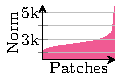
\includegraphics{figures/tikz/outliers_norms_no_regs.pdf}
 &
            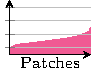
\includegraphics{figures/tikz/outliers_norms_registers.pdf}
 &  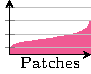
\includegraphics{figures/tikz/outliers_norms_att_bias.pdf}
 & 
             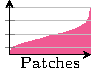
\includegraphics{figures/tikz/outliers_norms_value_gating.pdf}

             \\
            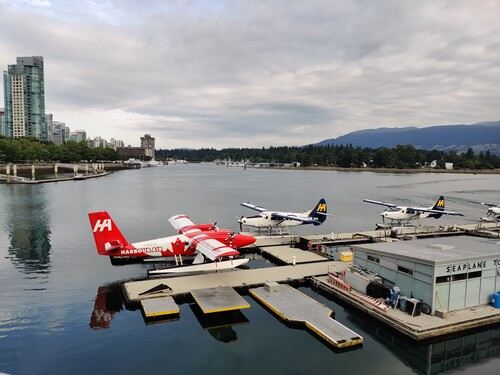
\includegraphics[height=2.1cm, width=2.1cm]{images/outliers/comparison/IMG_20250720_075113.lr.jpg} & 
            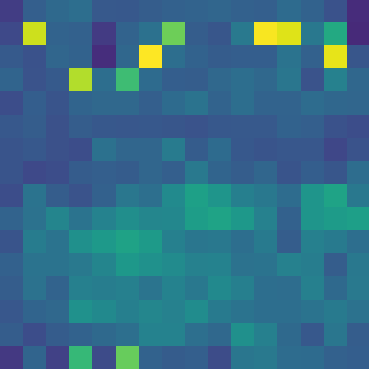
\includegraphics[height=2.1cm]{images/outliers/comparison/IMG_20250720_075113.jpg_registers_0_att_bias_False_value_gating_False_noLN.png} & 
            
\includegraphics[height=2.1cm]{images/outliers/comparison/IMG_20250720_075113.jpg_u1_untie_cp_False_gl_True_noLN.png} & 
            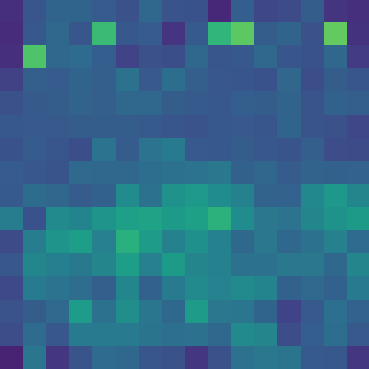
\includegraphics[height=2.1cm]{images/outliers/comparison/IMG_20250720_075113.jpg_registers_0_att_bias_True_value_gating_False_noLN.png} & 
            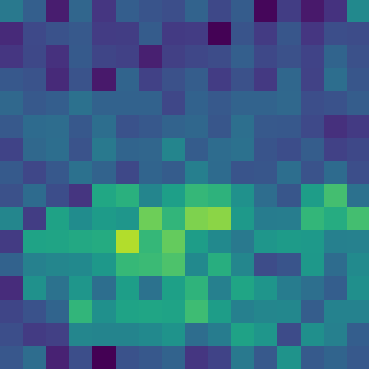
\includegraphics[height=2.1cm]{images/outliers/comparison/IMG_20250720_075113.jpg_registers_0_att_bias_False_value_gating_True_noLN.png}
            \\
            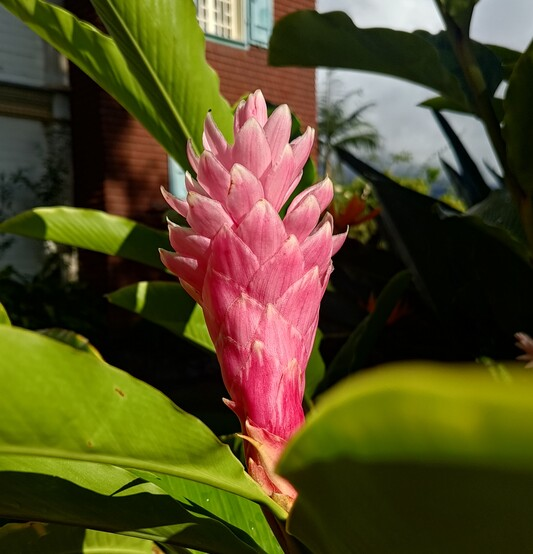
\includegraphics[height=2.1cm, width=2.1cm]{images/outliers/comparison/P_20250104_170117_crop.lr.jpg} &  
            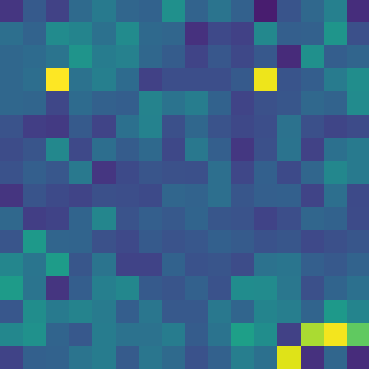
\includegraphics[height=2.1cm]{images/outliers/comparison/P_20250104_170117_crop.jpg_registers_0_att_bias_False_value_gating_False_noLN.png} &  
            
\includegraphics[height=2.1cm]{images/outliers/comparison/P_20250104_170117_crop.jpg_u1_untie_cp_False_gl_True_noLN.png} &  
            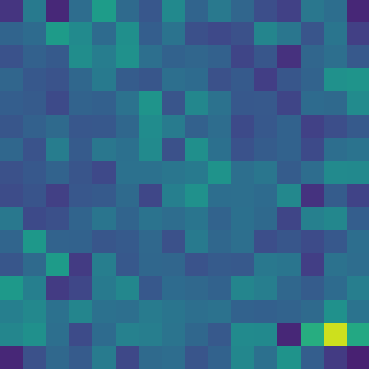
\includegraphics[height=2.1cm]{images/outliers/comparison/P_20250104_170117_crop.jpg_registers_0_att_bias_True_value_gating_False_noLN.png} &  
            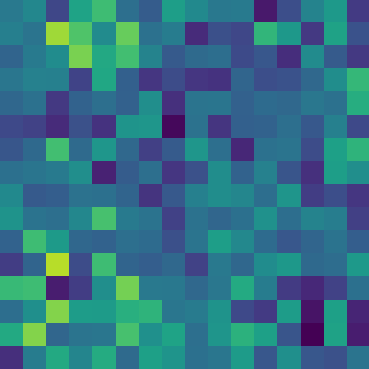
\includegraphics[height=2.1cm]{images/outliers/comparison/P_20250104_170117_crop.jpg_registers_0_att_bias_False_value_gating_True_noLN.png}
            \\
            \\
            Image & $\varnothing$ & 4 Registers & Attention  & Value  \\
             & & &  Bias &  Gating \\
        \end{tabular}
        \centering
        \caption{Visualization of patch norms by outlier strategy. The bottom two rows share a colormap per row, from dark blue (low) to yellow (high).}
        \label{fig:outliers-regis-attention}
    \end{subfigure}
    \hfill
    \begin{subfigure}{.33\linewidth}
        \centering
        \small
        \captionsetup{justification=centering}
        \caption{Quantitative ablation.}
        \label{tab:outliers-regis-attention}
        \addtolength{\tabcolsep}{-0.3em}
        \begin{tabular}{l c cc}
            Outlier &  & IN1k & ADE20k \\
            Strategy &  & (Linear) & mIoU \\
            \toprule
            $\varnothing$ & & 86.4 & \bf 53.2 \\
            4 Registers & & \bf 86.6 & 53.0 \\
            Attention Bias & & 86.5 & 52.7 \\
            Value Gating & & 86.3 & 52.2 \\
        \end{tabular}
        \vspace{5em}    
    \end{subfigure}
    \caption{Impact of the different strategies to mitigate the presence of high-norm patch outliers, evaluated both (a) qualitatively and (b) quantitatively. 
    We produce results with a 7B model trained with our recipe for 150k iterations, without any high-norm handling strategy `$\varnothing$', when using four register tokens \citep{darcet2024vision}, or the attention bias and value gating strategies \citep{an2025systematic}. 
    In (a, first row), we plot the distribution of the output patch norms (sorted by ascending values) computed for three images. We also visualize the output patch norms per image (bottom two rows), with the same colormap--min and max values are computed per image over the different outlier strategies. }
    \label{fig:outliers}
\end{figure}
 
\paragraph{Integrating Biases in the Attention Mechanism} 
Recent work by \citet{an2025systematic} investigates the appearance of outliers in the LLM realm across different models and architectures. The authors analyze different types of outliers which are observed to be intrinsically linked to the attention mechanism. They propose to mitigate the problem with several solutions from which we select two promising solutions which seem relevant and require minimal changes to the attention, specifically the explicit fixed bias, which we call `value gating', and the attention bias strategies.
The value gating strategy amounts to adding a learnable value bias $\mathrm{\bf v'} \in \mathbb{R}^d$ to the output of the attention, specifically by redefining the attention mechanism as 
\begin{equation}
    \mathrm{Attn}(Q,K,V; \mathrm{\bf k'}, \mathrm{\bf v'}) = \mathrm{softmax}(\frac{Q[K^T]}{\sqrt{d}})V + \mathrm{\bf v'}, 
    \label{eq:value-gatting}
\end{equation}
with $Q, K, V \in \mathbb{R}^{T\times d}$ the query, key, and value matrices and $d$ the dimensionality of the
hidden space. 
Alternatively, the attention bias, defined in \cref{eq:attn-bias}, consists in integrating two learnable bias terms $\mathrm{\bf k'}, \mathrm{\bf v'} \in \mathbb{R}^d$ in the keys and values matrices, respectively. It is defined as follows: 
\begin{equation}
    \mathrm{Attn}(Q,K,V; \mathrm{\bf k'}, \mathrm{\bf v'}) = \mathrm{softmax}(\frac{Q[K^T\mathrm{\bf k'}]}{\sqrt{d}}) \left[ \genfrac{}{}{0pt}{}{V}{\bf v'} \right]. 
    \label{eq:attn-bias}
\end{equation}
We observe in \cref{fig:outliers-regis-attention} that the value gating strategy substantially modifies the distribution of patch norms, resulting in generally higher norm values and the elimination of clear outliers. While the attention mechanism mitigates the presence of high-norm tokens, it does not completely resolve the issue, as some high-norm patches persist--as visible in the top row image--when compared to our results using register tokens. Notably, the best performance is achieved with the incorporation of the register tokens, which is why we adopt this strategy for all experiments reported is the paper.


\subsection{Feature Dimension Outliers}


The introduction of additional registers into the model architecture effectively resolves the issue of high-norm patch outliers. However, during the training of 7B models, we observe a distinct type of outlier that emerges not across patches, but within the feature (channel) dimension of the learned representations. Specifically, analysis of patch activations across transformer layers and training iterations reveals that a small subset of feature dimensions attain exceptionally large magnitudes, even as the norms across patches remain stable. Interestingly, these feature dimension outliers exhibit consistently high values across different patches and images, a behavior that contrasts with observations reported in \citep{an2025systematic}. Moreover, these outlier dimensions consistently persist across the layers of a given model, increasing in magnitude with depth and reaching their maximum values in the output layer. They also progressively increase in magnitude throughout the course of training.

We conduct experiments attempting to neutralize these dimensions during both training and inference. 
Our findings indicate that these dimensions play a significant role during training, as applying L2-regularization to suppress them results in a performance drop. 
However, removing these dimensions at inference time does not lead to significant performance changes, suggesting that they primarily carry trivial or non-informative signals. 
Additionally, we observe that the final layer normalization is trained to substantially scale down these outlier dimensions. 
Thus, we recommend to apply the final layer norm to the features of the final layer for downstream use.
Alternatively, applying batch normalization can also suppress these feature dimension outliers, as their elevated values are consistent across patches and images.

A word of caution applies to using features from earlier layers. 
As discussed above, these earlier layers are also affected by feature dimension outliers which can lead to ill-conditioned features.
While the final layer normalization is well-suited to normalize the distribution of the final features, its learned parameters may be suboptimal for applying it to the features of earlier layers. 
Indeed, we observe performance decreases for some tasks from doing so. 
In these cases, we found standard feature scaling techniques (\eg normalization with batch norm or principal component analysis) to be effective in dealing with the feature dimension outliers.
For example, for our semantic segmentation (\cref{sec:results-segmentation}) and depth estimation experiments (\cref{sec:results-depth-estimation}) using features from intermediate layers, we apply batch normalization.

 



